\documentclass{article}
\usepackage{nips2003e,times}
\usepackage[pdftex]{graphicx}
 \usepackage{fancyhdr,lastpage}	
\pagestyle{fancy}
\fancyhf{}
\rfoot{\scriptsize{Page \thepage}}
\renewcommand\headrulewidth{0pt} % Removes funny header line

\title{Forensic Signature Verification}
%\pagestyle{plain}

\author{
Apurva Sharma\\
Department of Computer Science\\
Georgia Institute of Technology\\
Atlanta, GA\\
\texttt{asharma70@gatech.edu} \\
\And
Parth Parekh\\
Department of Computer Science\\
Georgia Institute of Technology\\
Atlanta, GA\\
\texttt{parthparekh@gatech.edu} \\
\And
Urjit Singh Bhatia\\
Department of Computer Science\\
Georgia Institute of Technology\\
Atlanta, GA\\
\texttt{urjit.bhatia@gatech.edu} \\
}

% The \author macro works with any number of authors. There are two commands
% used to separate the names and addresses of multiple authors: \And and \AND.
%
% Using \And between authors leaves it to \LaTeX{} to determine where to break
% the lines. Using \AND forces a linebreak at that point. So, if \LaTeX{}
% puts 3 of 4 authors names on the first line, and the last on the second
% line, try using \AND instead of \And before the third author name.

\begin{document}

\maketitle

\begin{abstract}
This paper describes the implementation of a system that addresses the issues in the area of "Forensic Signature Verification". Two main approaches exist in this field- signature verification and signature identification. Our efforts focus on offline signature verification - the task of identifying whether a signature is genuine or forged given a genuine copy of the signature. Working on offline (static images) is a tougher task because temporal information which can provide key distinguishing features is missing. A part of our research focuses on trying to determine which are the key features which can help us discriminate between genuine and forged signatures and then developing algorithms which are able to do so from images of known genuine signatures and forgeries. Another focus area is on evaluating existing machine learning techniques against the extracted data sets and making suggestions for the same.

\end{abstract}

\section{Introduction}

This paper attempts to address the problems in the forensic handwriting examination domain. In particular, we focus our attention on verifying the authenticity of handwritten signatures. This research area holds great relevance in the judicial investigations. As the implications of this decision process are extremely critical; it is imperative that the false positives and false negatives are minimal. Because of such a precarious nature, currently verification is manually performed by signature experts having years of experience in this domain.

There are two key variations to the above problem - Signature authentication and Signature identification. Signature authentication is the task of authenticating whether the questioned signature is genuine or forged, given a genuine signature. In contrast, Signature identification processes the given signature sample and tries to predict who is the writer of that signature, given some information about the writers in the form of training samples. This subtle difference is better explained through the diagram below:

\begin{figure}[h]
\begin{center}
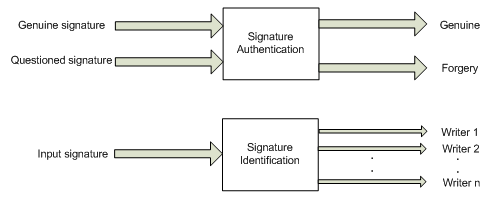
\includegraphics[width=5in,height=2in]{BlockDiagram.PNG}
\end{center}
\caption{Comparison of Authentication and Identification models}
\end{figure}

Writer identification requires that the handwriting samples of all the writers are known prior to identifying one amongst them. We realize this is often not the case. Authentication model on the other hand provides results that have statistical inference [1]. Another distinguishing factor relies on the way the data is collected - online or offline. On-line signature capture approaches typically employ devices like digital tablets which not only capture handwriting characteristics but also temporal characteristics which often provide very useful information. Capturing a signature offline is a lot simpler as all it requires is a pen and a paper. However, this makes authentication a harder problem as we lose the temporal information. In our study we have focused on datasets which collect information in an offline manner.

\begin{figure}[h]
\begin{center}
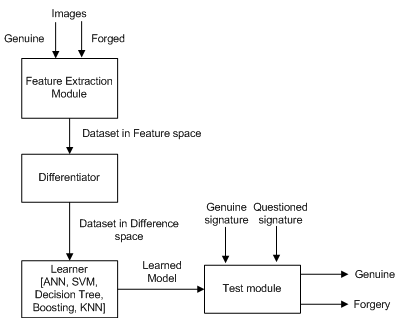
\includegraphics[width=5in,height=3.25in]{ProjectDiagram.PNG}
\end{center}
\caption{System architecture}
\end{figure}

We have attempted to implement an end-to-end system which employs a set of machine learning techniques to verify the authenticity of handwritten signatures. This system accepts images of a genuine and a questioned signature as input and tries to identify whether the questioned signature was authentic or a forgery. The diagram in Figure 2 shows the architecture of the system.

\section{Imageset Description}
For our research we have used the image data set made publicly available by Cedar Labs [2]. The data set is in the form of images of genuine and forged signatures. The dataset consists of signature samples taken from 55 people. For each person, there were 24 authentic and 24 forged samples, giving a total of 1320 genuine and 1320 forged signatures. All the images are assumed to have been written with the same pen, otherwise we run the risk of predicting whether the signatures were written from the same pen as opposed to whether the signatures were written by the same person. The background texture for all the signatures is plain white and it reduces overhead involved with tasks like line removal. The images are in png format and though they seem gray scale, actual image analysis revealed there was information in the RGB  channels too. These images are first converted to pure grayscale to ease processing.
Sample raw images for one pair of original and forged signatures and their corresponding processed images are shown in Figure 6.

\section{Feature selection and Extraction}
This is one of our key research focuses. The end performance of the system depends greatly on the choice of these attributes and how much discriminating power they have. After going through a lot of literature in the field [1],[3],[4],[5],[6] (amongst  many others) we were able to converge on some features that represent the individual idiosyncrasies of the signatures. These features can be divided into the following related groups:

1. Features based on the whole image (Macro Features)\\
2. Features based on the character level changes (Micro Features)\\
3. Features based on the DTW approach (Dynamic Time Warping)

We focused on macro features as they capture the most basic information required and many such features are utilized by existing Forensic Handwriting Experts too. DTW is also a very interesting approach that uses Zernike Moments to try and capture temporal like information for offline systems. However, we intend to work on these features in the future and add them to the set of features our system can currently extract and exploit.

The macro features we decided upon were broadly classified into the categories of measures of pen pressure, measure of writing movement, measures of stroke formation, slant and proportion. Figure 3 shows the classification of these features.

\begin{figure}[h]
\begin{center}
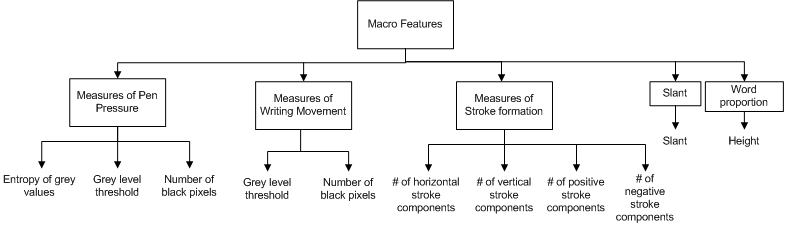
\includegraphics[width=5.75in,height=2in]{Features.png}
\end{center}
\caption{Features classification}
\end{figure}


These features and their extraction methods are discussed below:

\subsection{Measures of Pen-Pressure}

The following features capture the differences that arise in two signature samples due to pen-pressure. Angle-of-contact and speed are also closely related to this measure. For the same person, the pressure and speeds do not vary much. For example, it was observed from the data we generated, that the variance of the Grey Level Thresholds among original signature samples of the same person is 13.47 while that among originals and attempted forgeries for the same signature is 52.49.


\begin{table}[t]
\caption{Observed variance(s) for originals and forgeries for the measures-of-pen-pressure. This indicates that the originals are closer together and forgeries have larger differences (from the originals) as expected.\\}
\label{MOPP}
\begin{center}
\begin{tabular*}{0.75\textwidth}{@{\extracolsep{\fill}} | c | c | r | }
\hline
{\bf Features}         & {\bf Originals} & {\bf Forgeries} \\
\hline
Entropy                & 0.002514 & 0.036937 \\
\hline
Grey level threshold   & 13.47    & 52.49    \\
\hline
Number of black pixels & 1174007  & 2339116  \\
\hline
\end{tabular*}
\end{center}
\end{table}


\subsubsection{Entropy of gray values}

Entropy is an measure of disorder based on the information available in the images. The measure of entropy is useful for calculating and comparing the signature samples since entropy indicates to what degree writing styles vary for each writer. To find the entropy of gray values, we created a histogram over all the possible gray values that the pixels can take. Thus 256 bins are created and were populated with the frequency of the pixels having that gray value. Entropy was calculated using the formula: -1*p*log(p) where p was derived as p = (value in a bin)/(total number of pixels).

\subsubsection{Grey Level Threshold}

Grey level thresholding is used to classify pixels belonging to the image foreground and the image background. In the case of signature images, the foreground is the ink writing and the background is the paper. While the classification may seem obvious, looking at the images at a magnified scale, the edges of the lines contain pixels whose grey levels trail off into the background color rather than a sharp and sudden change. We used the Otsu algorithm [8] do determine the threshold value. According to the algorithm, the threshold value is derived by minimizing the inter-class variance and maximizing the intra-class variance where the class is split based on the threshold value k. The value of k is adjusted over many iterations using this algorithm and then used for further preprocessing as well as as a feature itself.

It is useful to use the threshold value k as a feature since it gives an indication of black pixel density and can help capture specific idiosyncrasies of the signature process that arise out of pressure, angle of contact between the pen and the paper surface, speed of performing the signature etc and higher values denote lighter pen pressure. For example, if the writer holds the pen in contact with the paper for a long time at approximately the same position, then more ink will be absorbed by the paper and less if the tip of the pen moves more quickly. This in-turn affects how the pixel values trail off. A similar effect is generated by pressure.

This effect is visible in the images below. The image on the left is a raw image while the image on the right is a preprocessed image. These image blocks were magnified by a factor of about 2000\% from the original size. During preprocessing, the images are converted into a two-color coded form, the pixels are either black or white based on their value with respect to the calculated threshold value. This mapping process is also called 'binarization'.

\begin{figure}[ht]
    \begin{minipage}[b]{0.5\linewidth}
        \centering
        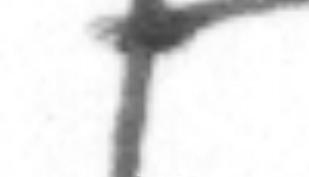
\includegraphics[width=1.25in, height=1in]{threshold2.png}
        \caption{Magnified raw image}
        \label{fig:figure1}
    \end{minipage}
    \hspace{0.5cm}
    \begin{minipage}[b]{0.5\linewidth}
        \centering
        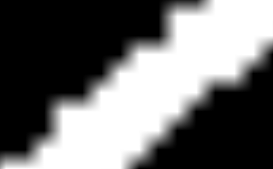
\includegraphics[width=1.25in, height=1in]{threshold1.png}
        \caption{Magnified preprocessed image}
        \label{fig:figure2}
    \end{minipage}
\end{figure}


\subsubsection{Number of Black Pixels}

This is a fairly straight forward measure. The number of pixels belonging to the class having grey values higher than the threshold are counted. This represents changes in writing due to varying pressure, thickness of the pen-tip and angle etc.

\subsection{Measures of Writing Movement}

Each image of handwritten signatures can be thought of as composed of blocks or blobs of connected sections [1]. These features measure changes along these blocks using chaincodes. We used Freeman Chain Codes spread in eight directions. Chaincodes give a sense of the direction in which the pixel densities change and thus a direction of movement of the pen strokes. The following features contain information about such directional changes:

\subsubsection{Number of Interior Contours}

The number of interior contours were found out by walking through the chain-codes generated for each connected block in the image. For each block, the inside edges form the interious contours and they are affected by the thickness of stroke and writing style. For example, large loops against small loops etc.

\subsubsection{Number of Exterior Contours}

Similar to the interior contours, the exterior contours are generated by counting the number of these contours formed by the outer edges of the strokes. Specific writing styles like cursive and block writing impact the number of interior and exterior contours formed while writing.

\subsection{Measures of Stroke Formation}

These features measure the proportion of characters and their general flow direction. Some people write all characters titled towards the front and some titled towards the back while some write straight characters.

\subsubsection{Number of Vertical Slope Components}

The vertical slope components were extracted by counting the number of chaincodes positioned with vertical orientations. Chaincodes with values 2 and 6 were used as vertical samples.

\subsubsection{Number of Horizontal Slope Components}

Similarly, the horizontal slope components were extracted by counting the number of chaincodes positioned with horizontal orientations, with values of 0 and 4.

\subsubsection{Number of Positive Slope Components}

The positive slope components are derived by counting the number of chaincodes pointing towards the first and the fourth quadrants.

\subsubsection{Number of Negative Slope Components}

The number of negative slope components was measured by counting the number of chaincodes pointing towards the second and the third quadrants.

\subsection{Slant}

The global slant determines the direction in which the words are written. The formula we used for finding the slant from the chaincodes is Slant s = atan((n1 - n3)/(n1 + numVerticalContours + n3)), where n1 and n3 are the number of diagonal components in the first, third and second, fourth quadrants respectively.

\subsection{Height}

We calculated the height of the signature to be determined by the height of its bounding box. A bounding box is an imaginary rectangle that bounds the extreme edges of the foreground pixels from all four sides. No point belonging to the foreground should lie outside this box. The height of the bounding box is found after performing image binarization.

A high level overview of Feature extraction process is shown in Figure 6.

\begin{figure}[h]
\begin{center}
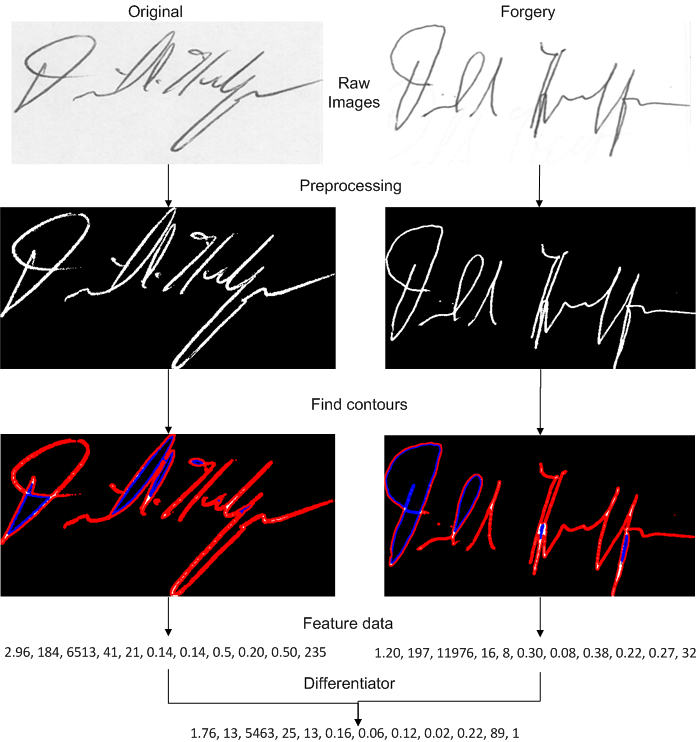
\includegraphics[width=5in,height=5in]{ImageProcessing.PNG}
\end{center}
\caption{Feature Extraction process}
\end{figure}


\section{Extracted Dataset Description}

Once the macro features are extracted, our problem is still an N-class problem (for N writers) as at this point, we can still only make predictions by comparing questioned signature with N  genuine signatures and predict which is the closest. However, there is a better approach which converts this to a 2-class categorization problem by making use of the fact that within writer distances are much less than between writer distances[1]. This though comes at the cost of explosion of the dataset. Till now, we had 2640 instances. However when we migrate the dataset to difference space, the number of instances increases to 46,860! (55* (24C2 +24*24)). This includes feature wise differences between all original signatures and all original and forged signatures. We keep the data set size in check by ignoring the intra class distances for the forged signatures as this is of no interest to us - we need not know how much two forgeries differ from each other.
\\
\\
\begin{figure}[ht]
	\begin{center}
        		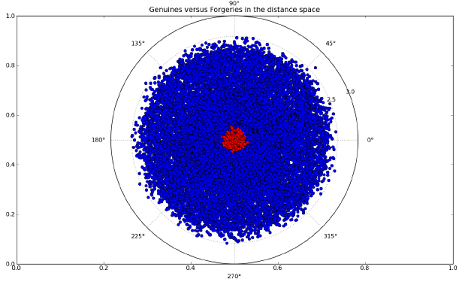
\includegraphics[width=2.5in, height=1in]{polarfigure.png}
       		 \caption{Polar plot of points in distance space. Red represents the inter-genuine distance points and Blue represents the genuine-forgery distance points}
	\end{center}
\end{figure}

\section{Evaluation}

We evaluated the system based on two different perspectives:

\subsection{Dataset generation}
Here we split the train and test data in two different ways:

\subsubsection{Divided on basis of authors}
The signatures from 55 people were split into test and train data on basis of authors. We created the entire training sample set of signatures (24 original, 24 forged) from each of the 30 writers. For testing purposes, we took samples (24 original, 24 forged) for each of the remaining 25 people. This approach had the advantage that no leakage of information from the training set to the test set was possible. As the system has never seen any data related to the 25 people in the test set, this was really the true and crucial test. To be useful, the system should work well enough on inputs it has never seen.

\subsubsection{Divided on basis of number of signatures from each person}
This is subtly different from 5.1.1, the training set contained signatures (12 original, 12 forged) from each of the 55 people. The test set consisted of the remaining signatures (12 original, 12 forged) of each of the 55 people. The motivation was to observe the effects of information leak and see if there is a huge disparity in results of obtained from the method described in 5.1.1 and the current approach and also find out what latent factors can cause possible information leak.

\subsection{The machine learning perspective}
For each of the training and test sets obtained in 5.1, we ran various machine learning algorithms to minimize the classification error. Following are the different algorithms that we ran on the datasets obtained by the configurations described above:

1. Decision Tree (J48)\\
2. K - Nearest Neighbors\\
3. Support Vector Machines (We used Poly kernels for this)\\
4. Neural Network\\
5. AdaBoost over SVMs\\
6. AdaBoost over Decision Tree (J48)\\

We ran all the above algorithms on the training data and generated models for it. We tested these models with the corresponding test data and found the best performing algorithm for both the scenarios. To boost the accuracy we clustered the original data (train + test) using the Expectation Maximization (EM) algorithm. The resulting cluster information was added as an additional feature to the datasets and the best performing algorithm, for both the scenarios, was then run on resultant dataset. Following graph shows the results for both the scenarios:

\begin{figure}[ht]
    \begin{minipage}[b]{0.5\linewidth}
        \centering
        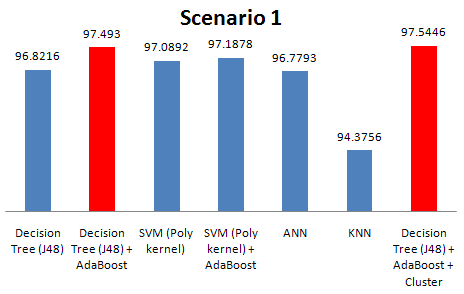
\includegraphics[width=2.5in, height=2in]{Test1.png}
        \caption{Scenario 1 results}
        \label{fig:figure1}
    \end{minipage}
    \hspace{0.5cm}
    \begin{minipage}[b]{0.5\linewidth}
        \centering
        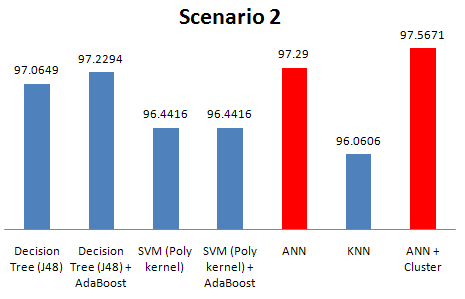
\includegraphics[width=2.5in, height=2in]{Test2.png}
        \caption{Scenario 2 results}
        \label{fig:figure2}
    \end{minipage}
\end{figure}

As it can be seen from the above graph that, AdaBoost over Decision tree gave the best result in scenario 1 and Neural network gave the best result for scenario 2. We clustered the data using EM algorithm and ran the same algorithms again to boost the accuracy. From the results it is evident that clustering does not seem to boost the accuracy much.

\begin{figure}[ht]
	\begin{center}
        		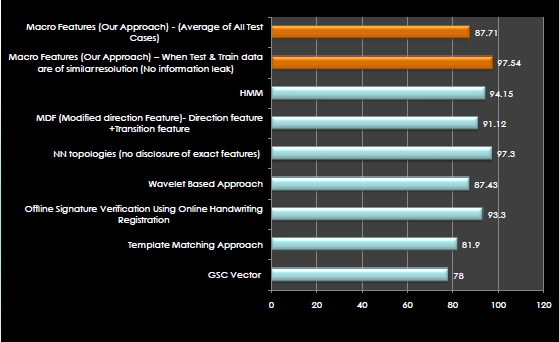
\includegraphics[width=4.5in, height=1.75in]{comparisons.png}
       		 \caption{Evaluation of various methods}
	\end{center}
\end{figure}

\section{Related Work}

There seems to have been a fair amount of interest in this field. CEDAR lab, in particular seems to do a lot of work in the handwriting domain with handwritten signatures receiving a fair amount of attention as well. Completely different approaches while targeting the same problem include wavelet based offline signature recognition [9], System Using HMM and Graphometric Features[10]. Other hybrid approaches [11] mix existing technologies like ANN's and HMM's. There are may other approaches too, which reaffirms our belief that this a particularly exciting and challenging problem to address.

\section{Conclusion}
The field of Forensic Signature Verification is in need for a scientific and objective basis. Our methods attempt to provide such a basis for signature verification. Using supervised machine learning techniques applied to the macro features holds potential, reaching an accuracy of 96\% and 83.5\% using models derived from low resolution image-set and a distinct high resolution image-set respectively. Aiding the current methods by feature space transformation (to the distance space), re-using clustering information and boosting gave promising results. During the course of the experiment, some very important observations were made - factors like image resolution affect how much information is captured. This becomes significant while building a model and these effects were clearly seen through the various testing scenarios. Given the highly subjective nature of this field, it becomes difficult to judge the accuracy of the system and the performance decreases if there is a lot of variance between the writers own genuine signatures, since in the distance space, they tend to move away from the 'average' signature. Offline signature verification is a particularly tricky problem, thus test cases need to be designed very carefully. Feature engineering as well as knowledge of which signatures were used as references are important points to consider while designing such a system.

\section{Future Work}

Future work for the project will be based on two major tracks:

\subsection{Domain Related}
This includes gaining more domain knowledge and find more features which can give much more discriminating information. Some of the features that are already being studied include GSC (Gradient, Structure, Concavity) vectors [1] and Zernike moments[8] which help in inferring temporal information for offline signatures. Also, some of the approaches mentioned in section 6 can be further explored.

\subsection{Machine Learning Related}
While we have already carried out evaluations with well established algorithms like Decision Trees, SVM's, kNN, Neural Nets with pretty good success, we can  explore other techniques like Hidden Markov Models which are known to have produced promising results in the area too.


\subsubsection*{Acknowledgments}

We are thankful to the Center of Excellence for Document Analysis and Recognition (CEDAR) group for providing the signature dataset. Our special thanks to Dr. Sargur Srihari for his strenous research in this domain and providing us with enough pointers to extract important features from the image data. Finally, we would like to thank Dr. Charles Isbell for guiding us throughout the process.


\subsubsection*{References}

\small{
[1] Srihari, S.N. \& Cha, S.H. \& Arora, H. \& Lee, S. {\it Individuality of Handwriting}, J Forensic Sci.

[2] Signature dataset - CEDAR, University at Buffalo, {\it http://www.cedar.buffalo.edu/NIJ/publications.html}

[3] Srihari, S.N. \& Chen, S. {\it Combining one and two dimensional signal recognition approaches to off-line signature verification}

[4] Ostu, N. {\it A Threshold Selection Method from Gray Level Histogram}, IEEE Trans. on
     Systems, Man and Cybernetics.

[5] Srihari, S.N. \& Cha, S-H. \& Arora, H. \& Lee, S. {\it Handwriting identification: research
to study validity of individuality of handwriting and develop computer-
assisted procedures for comparing handwriting}

[6] Favata, J.T. \& Srikantan, G. \& Srihari, S. N. {\it Handprinted Character/Digit Recognition using a Multiple Feature/Resolutio Philosophy}

[7] Xu, L. \& Krzyzak, A. \& Suen, C.Y. {\it Methods of combining multiple classifiers and their applications to handwriting recognition}

[8] Plamondon, R. \&  Srihari, S.N. \& Ecole P. \& Montreal, Q. {\it Online and off-line handwriting recognition: a comprehensive survey}

[9] Deng, P.S. \& Liao, H-Y.M. \& Ho, C.H. \& Tyan, H-R. {\it Wavelet�based Off�line Signature Verification}

[10] Edson J. R. J. \& Yacoubi A. El. \& Bortolozzi, F. \& Sabourin, R. {\it An Off-Line Signature Verification System Using HMM and Graphometric Features}

[11] Bourlard, H. \&  Morgan, N. {\it Hybrid HMM/ANN Systems for Speech Recognition: Overview and New Research Directions
}

\end{document}
